\section{Dika Sukma Pradana(1174050)}

\subsection{Koordinat}
\par
Koordinat adalah sistem koordinat yang memungkinkan setiap lokasi di Bumi ditentukan oleh serangkaian angka, huruf, atau simbol. Koordinat sering dipilih sedemikian sehingga salah satu angka mewakili posisi vertikal dan dua atau tiga angka mewakili posisi horisontal; sebagai alternatif, posisi geografis dapat diekspresikan dalam vektor Kartesius tiga dimensi. Pilihan umum koordinat adalah lintang, bujur dan ketinggian. Untuk menentukan lokasi di pesawat membutuhkan proyeksi peta. secara singkanya yaitu salah satu dari dua garis lintang dan bujur yang persimpangannya menentukan titik geografis suatu tempat.


\begin{figure}[H]
	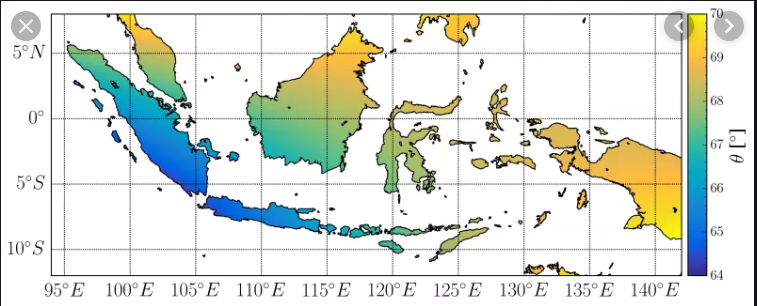
\includegraphics[width=4cm]{figures/1174050/koordinat.png}
	\centering
	\caption{Koordinat Indonesia}
\end{figure}

\subsection{Link}
\href{https://www.youtube.com/watch?v=GnI25H4HATo}{LINK Youtub, JANGAN LUPA SASKREB}
\subsection{Plagiarism}
\begin{figure}[H]
	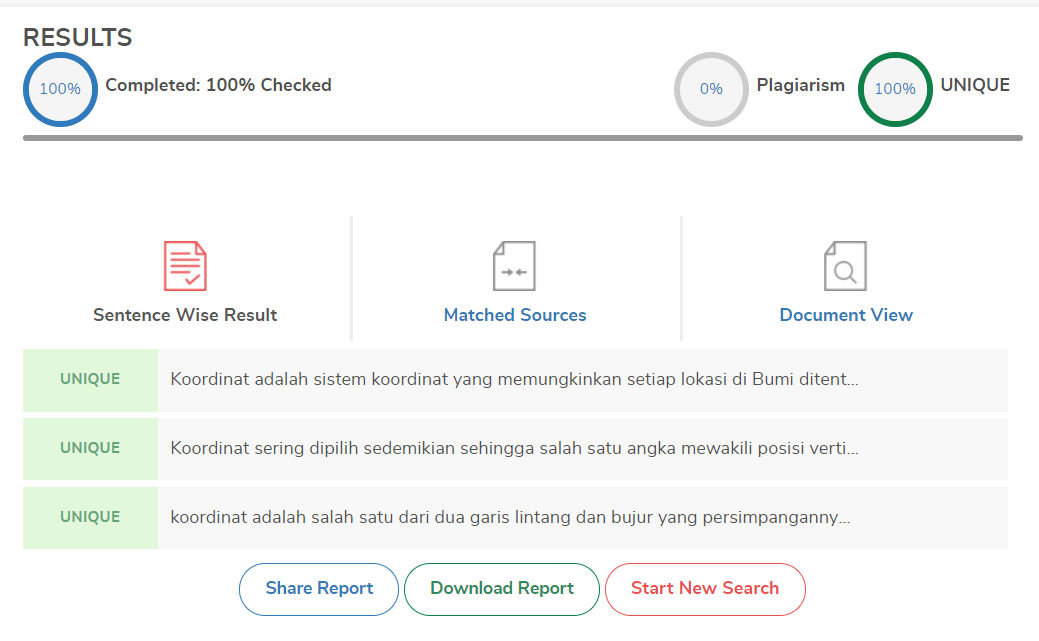
\includegraphics[width=4cm]{figures/1174050/plagiarism.png}
	\centering
	\caption{Plagiarism}
\end{figure}